\documentclass[11pt,a4paper]{article}
\usepackage[T1]{fontenc}
\usepackage[utf8]{inputenc}
\usepackage{lmodern}
\usepackage{amsmath,amssymb,amsthm,mathtools,mathrsfs}
\usepackage{graphicx,float,xcolor,multicol}
\usepackage[shortlabels]{enumitem}
\usepackage[margin=27mm]{geometry}
\usepackage{microtype,needspace,placeins}
\usepackage{tikz,tikz-cd}
\usetikzlibrary{arrows.meta,calc,positioning,patterns,decorations.pathreplacing}
\usepackage[colorlinks=true,linkcolor=teal,urlcolor=teal,citecolor=teal]{hyperref}
\setlength{\parindent}{0pt}
\setlength{\parskip}{.6em}
\setcounter{secnumdepth}{0}
\allowdisplaybreaks
\raggedbottom
\providecommand{\cross}{\times}
\DeclareUnicodeCharacter{2020}{\ensuremath{\dagger}}
\DeclareMathOperator{\supp}{supp}
\DeclareMathOperator*{\esssup}{ess\,sup}
\providecommand{\chapter}{\section}
\newenvironment{tool}[2]{\subsection*{Tool #1 --- #2}}{}
\newcommand{\ToolRef}[1]{Tool #1}
\newcommand{\FigureTag}[2]{\textit{Figure #1}}
\newcommand{\Result}[1]{\subsection*{#1}}
\newcommand{\Application}[1]{\subsubsection*{Application\if\relax\detokenize{#1}\relax\else\space--- #1\fi}}
\newcommand{\ProofHeading}{\par\textit{Proof.}\space}
\newcommand{\ProofOf}[1]{\par\textit{Proof of #1.}\space}
\newcommand{\RemarkHeading}{\par\textbf{Remark.}\space}
\newcommand{\NoteHeading}{\par\textbf{Note.}\space}
\newcommand{\ExerciseHeading}{\par\textbf{Exercise.}\space}

\graphicspath{{figures/complex-analysis/}}
\begin{document}
\section*{Goursat's Theorem and Cauchy's Theorem}
% BLOG-CONTENT-BEGIN
\subsection*{Tool 8 — Linear Approximation}
If $f$ is differentiable at $z_0$, then we have
\[
  f(z)=f(z_0)+f'(z_0)(z-z_0)+\psi(z),
  \qquad \psi(z)=o(z-z_0).
\]


\subsection*{Goursat's Theorem}
Let $T\subset U$ be the convex hull of $z_1,z_2,z_3$.
Then, if $f\colon U\to\mathbb C$ is holomorphic,
\[
  \int_{\partial T} f(z)\,dz=0,
\]
where $\partial T$ is the polygonal path
$\gamma_{z_1\to z_2\to z_3\to z_1}$.

\textit{Proof.}

\begin{figure}[htbp]
  \centering
  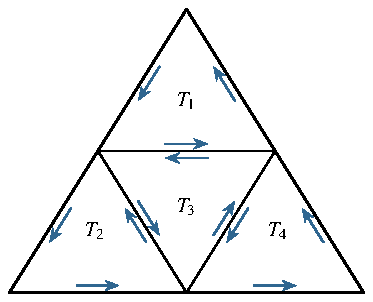
\includegraphics[width=.42\textwidth]{note3-fig-01.pdf}

\end{figure}

\begin{figure}[htbp]
  \centering
  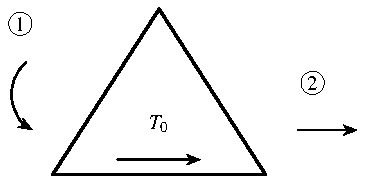
\includegraphics[width=.36\textwidth]{note3-fig-02.pdf}

\end{figure}

\begin{figure}[htbp]
  \centering
  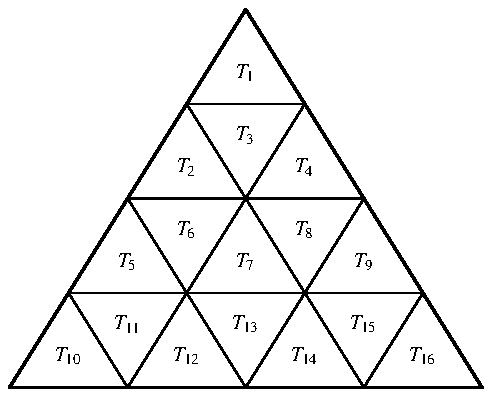
\includegraphics[width=.50\textwidth]{note3-fig-03.pdf}


\end{figure}


As the picture suggests,
\[
  \left|\int_{T_0}f(z)\,dz\right|
  \leq
  4\sup_{i\in\{1,2,3,4\}}
  \left|\int_{T_i}f(z)\,dz\right|,
\]
and, further, we can repeat the argument for $T_i$ (say $T_1$, without loss of
generality) to obtain
\[
  \left|\int_{T_0}f(z)\,dz\right|
  \leq 4\left|\int_{T_1}f(z)\,dz\right|
  \leq 4^2\left|\int_{T_2}f(z)\,dz\right|
  \leq\cdots\leq
  4^n\left|\int_{T_n}f(z)\,dz\right|
\]
after $n$ stages. Now one has to compensate for the $4^n$.
Note first that the $T_n$, seen as solid triangles, are compact sets and
$T_n\supseteq T_{n+1}$, so
\[
  \bigcap_n T_n=\{z_0\}
\]
for some $z_0$ in the solid triangle $T_0$. Now let us approximate $f$ around
$z_0$:
\[
  f(z)=f(z_0)+f'(z_0)(z-z_0)+\psi(z)(z-z_0),
  \qquad \psi(z)\to0\quad\text{as }z\to z_0.
\]
Note that $f(z_0)$ and $f'(z_0)(z-z_0)$ have primitives. Therefore, we
essentially have
\[
  \int_{T_n}f(z)\,dz
  =\int_{T_n}\psi(z)(z-z_0)\,dz.
\]
Let $d_n$ be the diameter of $T_n$ and $p_n$ its perimeter. Then
\[
  d_n=\frac{d_0}{2^n},
  \qquad
  p_n=\frac{p_0}{2^n},
\]
and hence
\[
  \left|\int_{T_n}\psi(z)(z-z_0)\,dz\right|
  \leq \int_{T_n}|\psi(z)(z-z_0)|\,|dz|
  \leq \frac{\varepsilon_n d_0p_0}{4^n},
  \qquad
  \varepsilon_n=\sup_{z\in T_n}|\psi(z)|.
\]
Thus the error in the linear approximation helps us compensate for the $4^n$:
\[
  \left|\int_{T_0}f(z)\,dz\right|
  \leq 4^n\left|\int_{T_n}f(z)\,dz\right|
  \leq 4^n\left(\frac{\varepsilon_n d_0p_0}{4^n}\right)
  \leq \varepsilon_n d_0p_0.
\]
Let $n\to\infty$. Since $\varepsilon_n\to0$,
\[
  \int_{T_0}f(z)\,dz=0.
\]

\textbf{Remark.}
Holomorphicity at every point is unnecessary here. Suppose that $f$ is merely
bounded near a point $z_0$ in the solid triangle. By subdividing the triangle
as illustrated below, one may reduce to the case in which $z_0$ is a vertex.

\begin{figure}[H]
  \begin{minipage}[t]{.48\textwidth}
    If $z_0$ is in the interior of $T_0$,\par
    \begin{minipage}[c][5.1cm][c]{\linewidth}
      \centering
      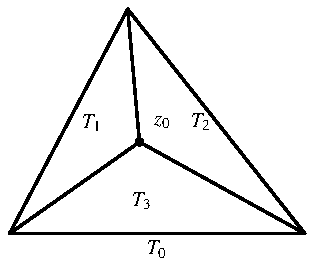
\includegraphics[width=.708\linewidth]{note3-fig-04.pdf}
    \end{minipage}


  \end{minipage}
  \begin{minipage}[t]{.48\textwidth}
    If $z_0$ is on $T_0$,\par
    \begin{minipage}[c][5.1cm][c]{\linewidth}
      \centering
      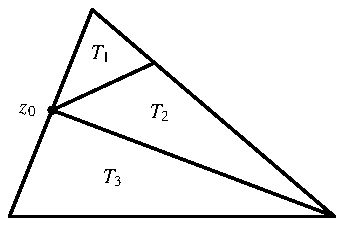
\includegraphics[width=.792\linewidth]{note3-fig-05.pdf}
    \end{minipage}


  \end{minipage}
\end{figure}

Now we know that $z_0$ is a vertex:
\begin{figure}[H]
  \begin{minipage}[b]{.48\textwidth}
    \begin{minipage}[c][5.0cm][c]{\linewidth}
      \centering
      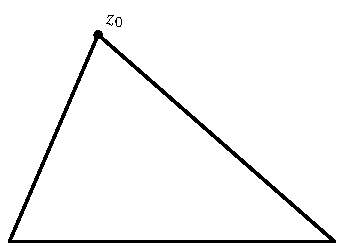
\includegraphics[width=.708\linewidth]{note3-fig-06.pdf}
    \end{minipage}

  \end{minipage}
  \begin{minipage}[b]{.48\textwidth}
    \begin{minipage}[c][5.0cm][c]{\linewidth}
      \centering
      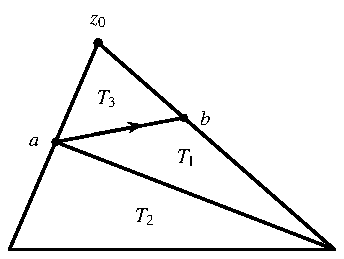
\includegraphics[width=.792\linewidth]{note3-fig-07.pdf}
    \end{minipage}

  \end{minipage}
\end{figure}

For all $a,b\neq z_0$, on $T_1$ and $T_2$ the integral will vanish; and, since
$f$ is bounded near $z_0$, the integral on $T_3$ can be made arbitrarily small,
as the perimeter can be made very small. Also note that what we essentially
need to prove Goursat's Theorem is a linear form as given below. For every
$z_0$,
\[
  f(z)=a_{z_0}+b_{z_0}(z-z_0)+\psi_{z_0}(z)(z-z_0)
  \qquad\text{on }U\setminus\{z_0\},
\]
where $\psi_{z_0}(z)\to0$ as $z\to z_0$.

Observe immediately that holomorphic functions except on a discrete set, where
they have removable discontinuities, are candidates. Thus Goursat's Theorem
works for a wider class of functions than merely holomorphic functions.


\subsubsection*{Application — Holomorphic primitives on convex domains}
Let $f$ be holomorphic on an open, connected, convex set.
Then $f$ has a primitive; that is, there exists $F$, holomorphic on the same
convex domain, such that $F'=f$.

\textit{Proof.}
Let $\Omega$ be the domain, and fix $z_0\in\Omega$. Define
\[
  F(z):=\int_{\gamma_{z_0\to z}}f(z)\,dz.
\]

\begin{figure}[htbp]
  \centering
  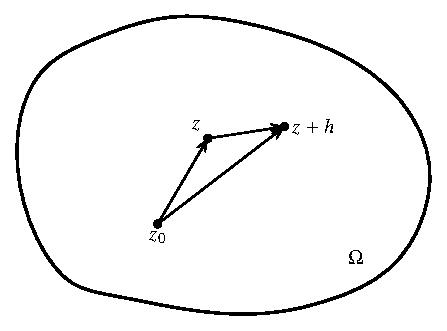
\includegraphics[width=.46\textwidth]{note3-fig-08.pdf}

\end{figure}

By Goursat's Theorem, we have
\[
  F(z+h)-F(z)=\int_{\gamma_{z\to z+h}}f(z)\,dz.
\]
For $f$ at $z$, we have
\[
  f(w)=f(z)+f'(z)(w-z)+\psi(w).
\]
Therefore,
\begin{align*}
  F(z+h)-F(z)
  &=\int_{\gamma_{z\to z+h}}f(z)\,dw
    +\int_{\gamma_{z\to z+h}}f'(z)(w-z)\,dw
    +\int_{\gamma_{z\to z+h}}\psi(w)\,dw\\
  &=f(z)h+f'(z)\left(\frac{w^2}{2}-wz\right)\Big|_z^{z+h}
    +\int_{\gamma_{z\to z+h}}\psi(w)\,dw\\
  &=f(z)h+f'(z)\left(
      \frac{(z+h)^2}{2}-(z+h)z-\left(\frac{z^2}{2}-z^2\right)
    \right)
    +\int_{\gamma_{z\to z+h}}\psi(w)\,dw\\
  &=f(z)h+\frac{f'(z)h^2}{2}
    +\int_{\gamma_{z\to z+h}}\psi(w)\,dw.
\end{align*}
This gives a second-order Taylor approximation for $F$. Note that
\[
  \left|\int_{\gamma_{z\to z+h}}\psi(w)\,dw\right|
  \leq \sup_{w\in\gamma_{z\to z+h}}|\psi(w)|,
\]
which goes to $0$ as $h\to0$. Hence
\[
  \lim_{h\to0}\frac{F(z+h)-F(z)}{h}=f(z).
\]


\subsection*{Tool 9 — Complex Tube Lemma}
Given any continuous curve in a domain $\Omega$, there exists a polygonal path
``close'' to the curve.


\textbf{Note.}
These polygons are useful, for one can invoke Goursat's Theorem. In fact, we can
say something more: if there is a convex set $U\subset\Omega$ such that the
continuous curve and its polygonal ``approximation'' both lie in $U$, then the
polygonal path and the curve form a closed continuous curve in $U$. If,
moreover, we demand that $\gamma$ be rectifiable, then
\[
  \int_\gamma f(z)\,dz=\int_P f(z)\,dz
  \qquad\bigl(\forall f, f\in H(\Omega)\bigr),
\]
where $P$ is the polygonal path. This is because $f$ has a primitive in $U$, as
was seen previously.

\begin{figure}[htbp]
  \centering
  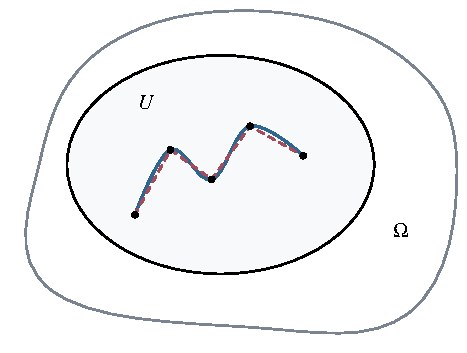
\includegraphics[width=.52\textwidth]{note3-fig-09.pdf}

\end{figure}

\subsection*{Cauchy's Theorem}
Let $f\in H(U)$, where $U$ is a domain, and let $\gamma_0$ and $\gamma_1$ be
rectifiable and homotopic in $U$. Then
\[
  \int_{\gamma_0}f(z)\,dz=\int_{\gamma_1}f(z)\,dz.
\]

It is worth mentioning two important corollaries of Cauchy's Theorem, which are
more useful than the theorem itself.

\subsection*{Tool 10 — Cauchy Integral Formula}
\[
  f(z_0)=\frac{1}{2\pi i}\int_{C_R}\frac{f(z)}{z-z_0}\,dz.
\]
Here $f\in H(\Omega)$, and $C_R$ is a circle of radius $R$ such that
$\operatorname{int}C_R\cup C_R\subset\Omega$.


\subsection*{Tool 11 — Higher-Order Cauchy Integral Formula}
\[
  f^{(n)}(z_0)=\frac{n!}{2\pi i}
  \int_{C_R}\frac{f(z)}{(z-z_0)^{n+1}}\,dz.
\]


\subsection*{Tool 12 — Local Analyticity}
\[
  f(z)=\sum_{n\geq0}\frac{f^{(n)}(z_0)}{n!}(z-z_0)^n
  \qquad\bigl(\forall z_0, z\in\operatorname{int}C_R\bigr).
\]

Tool 12 follows from Cauchy's integral formulas, Tools 10 and 11.
\subsubsection*{Application — Consequences of Cauchy's formulas}
The following applications of Tools 10, 11, and 12 may seem
standard, but they record useful consequences worth
recalling.


\subsection*{Tool 13 — Identity Theorem}

Let $f\in H(\Omega)$. If $z_n\to z_0$ in $\Omega$ and $f(z_n)=0$, then
$f\equiv0$.


\textit{Proof.}
Locally around $z_0$,
\[
  f(z)=\sum_n a_n(z-z_0)^n.
\]
Thus
\[
  f(z)=a_m(z-z_0)^m\bigl(1+g(z-z_0)\bigr),
\]
where $m$ is the least index such that $a_m\neq0$. Since
$g(z-z_0)\to0$ as $z\to z_0$, there exists $K$ such that, for every $k\geq K$, \(|g(z_k-z_0)|<1.\)
Therefore
\[
  a_m(z_k-z_0)^m\neq0
  \quad\text{and}\quad
  1+g(z_k-z_0)\neq0,
\]
but $f(z_k)=0$, a contradiction. Hence such an $m$ does not exist, so
$f(z)\equiv0$ locally. Now note that the set of points
$\{z\mid f(z)=0\}$ is closed. Hence the continuity method would force
$f\equiv0$.

\subsection*{Morera's Theorem}
Let $f$ be a continuous function on $\Omega$, and suppose that, for every
closed polygonal path $P$,
\[
  \int_P f(z)\,dz=0.
\]
Then $f\in H(\Omega)$.

\textit{Proof.}
Modify the ``existence of a primitive on a convex set'' proof and construct a
primitive for $f$. Let $F'=f$. Since $F\in H(\Omega)$ is locally analytic,
$f$ is locally analytic, and hence $f\in H(\Omega)$.

\textbf{Remark.}
Compare this with the Looman--Menchoff Theorem, which just demands the
Cauchy--Riemann equations along with continuity. Which is stronger?


\subsubsection*{Application — Polynomial characterization}
Let $f$ be entire such that, for each $z_0$,
$f^{(n)}(z_0)=0$ for some $n$. Then $f$ is a polynomial.

\textit{Proof.}
For every $z_0\in\mathbb C$, $f^{(n)}(z_0)=0$ for some $n$. By the
Pigeonhole Principle, for a fixed $n$, $f^{(n)}(z_0)=0$ for uncountably many
$z_0$. Thus the zero set of $f^{(n)}$ has a limit point in some disc, and
hence \(f^{(n)}(z)\equiv0.\)
Therefore $f$ is a polynomial, because
\[
  f(z)=\sum_{n=0}^{\infty}c_n(z-z_0)^n,
  \qquad
  c_n=\frac{f^{(n)}(z_0)}{n!},
\]
where $z_0$ is a zero of $f$. Hence, for every $m\geq n$, \(\frac{f^{(m)}(z_0)}{n!}=0.\)
Thus $f$ is locally a polynomial, and, by the Identity Theorem, $f$ is globally
a polynomial.

\textbf{Remark.}
The local power-series expansion about a point converges up to the
nearest point of singularity.
% BLOG-CONTENT-END
\end{document}
